% Draft for Optimization Letters (Springer).
% Written in standard article class for review; retarget to sn-jnl.cls
% (Springer Nature) at submission time -- content carries over unchanged.
\documentclass[11pt]{article}

\usepackage[margin=1in]{geometry}
\usepackage[T1]{fontenc}
\usepackage{lmodern}
\usepackage{amsmath,amssymb,amsthm,mathtools}
\usepackage{algorithm}
\usepackage{algpseudocode}
\usepackage{graphicx}
\usepackage{booktabs}
\usepackage[numbers,sort&compress]{natbib}
\usepackage{microtype}
\usepackage[hidelinks]{hyperref}

\newtheorem{theorem}{Theorem}
\newtheorem{lemma}{Lemma}
\newtheorem{proposition}{Proposition}
\newtheorem{corollary}{Corollary}
\theoremstyle{remark}
\newtheorem{remark}{Remark}

\newcommand{\R}{\mathbb{R}}
\newcommand{\supp}{\operatorname{supp}}
\newcommand{\Val}{\operatorname{Val}}
\newcommand{\T}{{\mathsf T}}
\newcommand{\prob}[1]{\mathrm{P}(#1)}

\title{Exactness of an iterated divide-and-conquer method for
large-scale nonnegative least squares}

\author{Emre H. Brookes\\[2pt]
\small Department of Chemistry \& Biochemistry, University of Montana,
Missoula, Montana, USA\\
\small \texttt{emre.brookes@umontana.edu}\ \ $\cdot$\ \ ORCID:
\href{https://orcid.org/0000-0001-7348-6476}{0000-0001-7348-6476}}

\date{\today}

\begin{document}
\maketitle

\begin{abstract}
Model-based fitting of experimental data frequently leads to nonnegative
least squares (NNLS) problems whose design matrices exceed the memory of a
single workstation; in the analysis of analytical ultracentrifugation
experiments, grids of up to $1.5\times10^{6}$ basis functions arise. A
divide-and-conquer method introduced at SC'06 addresses this bottleneck:
the parameter set is partitioned, NNLS is solved on each block, the
supports of the block solutions are unioned and re-solved, and, in an
iterative variant, the support of the final solution is fed back into
every block and the procedure repeated until the result no longer varies.
The iterative variant has been in production use in the UltraScan
software for two decades and has been observed to reproduce the
full-grid solution; however, a proof has been lacking. We prove that,
provided each subproblem is solved exactly and merge steps union whole
supports, the iterated scheme terminates after finitely many rounds at a
global minimizer of the full problem, for every partition sequence and
merge topology, and that the implemented stopping rule is a sound
certificate of global optimality. The optimal value and fitted vector
always coincide with those of the full computation; the solution itself
coincides under a standard uniqueness condition. A four-column
counterexample shows that the non-iterated scheme can be suboptimal by a
constant factor of the signal, so the feedback rounds are necessary.
Suboptimality under inexact pricing is bounded, and the analysis is
confirmed numerically on correlated designs representative of the
motivating application.
\end{abstract}

\noindent\textbf{Keywords:} nonnegative least squares $\cdot$ divide and
conquer $\cdot$ column generation $\cdot$ active-set methods $\cdot$
global optimality certificate $\cdot$ analytical ultracentrifugation

\medskip
\noindent\textbf{MSC codes:} 90C20 $\cdot$ 65F20 $\cdot$ 90C06 $\cdot$
65K05

\section{Introduction}\label{sec:intro}

Nonnegative least squares (NNLS) is a workhorse of model-based data
analysis: whenever measured data are represented as a nonnegative linear
combination of physically meaningful basis functions, the amplitudes are
determined by solving
\begin{equation*}
\min_{x\ge 0}\ \tfrac12\lVert Ax-b\rVert_2^2,
\end{equation*}
classically by the active-set algorithm of Lawson and
Hanson~\cite{lawson1974} and its accelerated
descendants~\cite{bro1997,vanbenthem2004,kim2011}. In the sedimentation
velocity analysis of analytical ultracentrifugation (AUC) data, each
column of $A$ is a finite-element solution of the Lamm equation for one
candidate solute, the grid ranges over sedimentation and frictional
parameters, and nonnegativity reflects physical concentrations; the
two-dimensional spectrum analysis (2DSA) implemented in
UltraScan~\cite{demeler2005,brookes2010} solves such problems routinely.

In practice the resolution of the analysis is limited less by the solver
than by memory: grids of $10^{5}$--$10^{6}$ basis functions exceed the
capacity of a single workstation. The divide-and-conquer method of
Brookes, Boppana and Demeler~\cite{brookes2006}, introduced at SC'06 and
deployed in UltraScan since, addresses this constraint directly. The
parameter set is partitioned into blocks; NNLS is applied to each block;
the supports of the block solutions --- the parameters that contribute to
each best fit --- are unioned, possibly in several stages, and NNLS is
applied to the union. Because a parameter discarded inside one block may
nevertheless be required by the full solution, the authors observed that
this basic scheme and the full computation ``usually
differ''~\cite{brookes2006}, and introduced an iterative variant: the
support of the final solution is unioned back into every block and the
procedure is repeated until the result no longer varies. Empirically the
iterative variant was found to be in exact correspondence with the
full-grid solution, typically within 3--7 rounds~\cite{brookes2006}, and
two decades of production use on cluster hardware are consistent with
that observation. A proof, however, has been lacking: the equivalence
underlying routine scientific results has rested on empirical evidence.

This note closes that gap. The contributions are:
\begin{enumerate}
\item[(i)] a proof that the iterated scheme terminates after finitely
many rounds at a global minimizer of the full problem, for arbitrary
per-round partitions (the moving-grid partitions of~\cite{brookes2006}
included) and arbitrary merge topologies, under two natural conditions:
subproblems are solved exactly, and merge steps union \emph{whole}
supports (Theorem~\ref{thm:main});
\item[(ii)] soundness of the implemented stopping rule: a round that
leaves the result unchanged certifies global optimality
(Theorem~\ref{thm:main}); the optimal value, fitted vector, and residual
then coincide with the full computation unconditionally, and the
amplitude vector itself coincides under a standard uniqueness condition
(Theorem~\ref{thm:outputs});
\item[(iii)] a four-column counterexample showing that the non-iterated
scheme can return a residual larger than the optimum by a constant
factor of the signal, so the feedback rounds are necessary rather than
cosmetic (Proposition~\ref{prop:counter});
\item[(iv)] a suboptimality bound of $\delta\lVert x^*\rVert_1$ when the
pricing test is satisfied only to tolerance $\delta$
(Proposition~\ref{prop:inexact}); and
\item[(v)] numerical confirmation on correlated designs representative
of the motivating application, including per-node verification of every
monotonicity inequality used in the proof (Section~\ref{sec:numerics}).
\end{enumerate}

The analysis places the method in a classical lineage. The refinement
round is a distributed \emph{pricing} step in the sense of column
generation~\cite{dantzig1960,gilmore1961}: the merged problem is a
restricted master, and the blocks jointly price every column of the full
grid against the current residual. The strict-improvement argument is
the same device that underlies convergence proofs for working-set
decomposition methods in support vector machine
training~\cite{osuna1997,lin2001}. What the present setting adds is the
merge-tree structure with changing partitions, an exact finite
termination argument (the objective values live in a finite set, so
strict descent cannot continue indefinitely), the certificate soundness
statement, and the counterexample delimiting the non-iterated scheme.
Notably, no bound on the working-set size must be imposed: NNLS supports
returned by active-set solvers are automatically bounded by the rank of
$A$, which is what keeps the merge stages small in practice.

Section~\ref{sec:prelim} fixes notation and collects preliminaries;
Section~\ref{sec:alg} formalizes the algorithm;
Section~\ref{sec:main} proves the main results;
Section~\ref{sec:counter} gives the counterexample;
Section~\ref{sec:inexact} treats inexact pricing;
Section~\ref{sec:numerics} reports the numerical checks; and
Section~\ref{sec:discussion} discusses implementation guidance,
limitations, and extensions.

\section{Problem and preliminaries}\label{sec:prelim}

Throughout, $A\in\R^{m\times n}$ has columns $a_j$ indexed by
$S=\{1,\dots,n\}$, and $b\in\R^m$. For $C\subseteq S$ the restricted
problem is
\begin{equation}\label{eq:pc}
\prob{C}:\qquad \min\ F(x):=\tfrac12\lVert Ax-b\rVert_2^2
\quad\text{s.t.}\quad x\ge 0,\ \supp(x)\subseteq C,
\end{equation}
with optimal value $\Val(C)$; the full problem is $\prob{S}$ with value
$v^*:=\Val(S)$. The residual is $r(x):=b-Ax$. Following the set-function
notation of~\cite{brookes2006}, $f(C):=\supp(x_C)$ denotes the support
of a minimizer $x_C$ of $\prob{C}$; when $\prob{C}$ has several
minimizers, $f$ may return the support of any one of them, and every
statement below holds for an arbitrary selection.

\begin{lemma}[existence; uniqueness of the fit]\label{lem:exist}
$\prob{C}$ attains its minimum, and $Ax_C$ is the same for every
minimizer $x_C$.
\end{lemma}
\begin{proof}
$K_C:=\{Ax:\ x\ge0,\ \supp(x)\subseteq C\}$ is a finitely generated
convex cone, hence closed \cite[Ch.~7]{schrijver1986}. The projection
$p_C$ of $b$ onto the closed convex set $K_C$ exists and is unique;
minimizers of $\prob{C}$ are exactly the feasible preimages of $p_C$.
\end{proof}

\begin{lemma}[optimality conditions]\label{lem:kkt}
A feasible $x$ solves $\prob{C}$ if and only if, with $r=r(x)$,
\begin{equation}\label{eq:kkt}
a_j^{\T}r\le 0\ \ \forall j\in C
\qquad\text{and}\qquad
a_j^{\T}r=0\ \ \forall j\in\supp(x).
\end{equation}
\end{lemma}
\begin{proof}
$F$ is convex and differentiable with $\nabla F(x)=-A^{\T}r$, and the
feasible set of \eqref{eq:pc} is convex, so $x$ is optimal iff
$(A^{\T}r)^{\T}(y-x)\le0$ for every feasible $y$. Choosing $y=x+e_j$
for $j\in C$ gives $a_j^{\T}r\le0$; choosing $y=x-x_je_j$ for
$x_j>0$ gives $a_j^{\T}r\ge0$, hence equality on the support.
Conversely, under \eqref{eq:kkt}, for any feasible $y$,
$(A^{\T}r)^{\T}(y-x)=\sum_{j\in C}(a_j^{\T}r)\,y_j\le0$, and convexity
gives $F(y)\ge F(x)$.
\end{proof}

\begin{lemma}[pricing]\label{lem:pricing}
If $x$ solves $\prob{C}$ and $a_j^{\T}r(x)\le0$ for all $j\notin C$,
then $x$ solves $\prob{S}$.
\end{lemma}
\begin{proof}
The conditions \eqref{eq:kkt} hold for $C=S$.
\end{proof}

The quantity $a_j^{\T}r$ is the negative reduced gradient of column
$j$; Lemma~\ref{lem:pricing} states that the full grid never needs to be
\emph{solved}, only \emph{priced}. This is the mechanism the iterated
method exploits.

\begin{lemma}[restriction]\label{lem:restrict}
\emph{(i)} If $C\subseteq C'$ then $\Val(C')\le\Val(C)$.
\emph{(ii)} If $x_C$ solves $\prob{C}$ and
$\supp(x_C)\subseteq D\subseteq C$, then $x_C$ solves $\prob{D}$ and
$\Val(D)=\Val(C)$.
\end{lemma}
\begin{proof}
(i) Feasible sets nest. (ii) The conditions \eqref{eq:kkt} for $D$ are a
subset of those for $C$.
\end{proof}

Lemma~\ref{lem:restrict}(ii) is why discarding zero-amplitude parameters
loses nothing about the \emph{current} solution; the risk --- and the
reason a proof is required --- is that a discarded parameter may be
needed by a \emph{better} solution not representable inside the block
where it was discarded. Section~\ref{sec:counter} shows this risk is
real.

\section{The divide-and-conquer method}\label{sec:alg}

Algorithm~\ref{alg:round} states one round in the notation
of~\cite{brookes2006}; Algorithm~\ref{alg:iter} states the iteration.
Round $k$ receives the incumbent result set $R_{k-1}$ (with
$R_0=\varnothing$) and produces the iterate $x_k$; the round with
$R_0=\varnothing$ is exactly the basic (non-iterated) scheme of
\cite[Text~1]{brookes2006}, and the loop of Algorithm~\ref{alg:iter} is
the iterative variant of \cite[\S3.2]{brookes2006}.

\begin{algorithm}[t]
\caption{One round of divide-and-conquer NNLS}\label{alg:round}
\begin{algorithmic}[1]
\Require incumbent set $R\subseteq S$; partition $S_1,\dots,S_p$ of $S$;
merge tree $\mathcal T$ with $p$ leaves
\For{$i=1,\dots,p$ (in parallel)}
  \State $y_i\gets$ minimizer of $\prob{S_i\cup R}$;\quad
         $U_i\gets\supp(y_i)$
\EndFor
\For{each internal node $\nu$ of $\mathcal T$, leaves upward}
  \State $C_\nu\gets\bigcup_{\mu\ \text{child of}\ \nu}U_\mu$;\quad
         $z_\nu\gets$ minimizer of $\prob{C_\nu}$;\quad
         $U_\nu\gets\supp(z_\nu)$
\EndFor
\State\Return $x\gets z_{\mathrm{root}}$,\ \ $R'\gets U_{\mathrm{root}}$,
\ \ $C\gets C_{\mathrm{root}}$
\end{algorithmic}
\end{algorithm}

\begin{algorithm}[t]
\caption{Iterated divide-and-conquer NNLS}\label{alg:iter}
\begin{algorithmic}[1]
\State $R_0\gets\varnothing$
\For{$k=1,2,\dots$}
  \State $(x_k,R_k,C_k)\gets$ Algorithm~\ref{alg:round} on $R_{k-1}$
         with the round's partition and tree;\quad $v_k\gets F(x_k)$
  \If{$k\ge2$ and the result is unchanged (or $v_k=v_{k-1}$)}
     \State\Return $x_k$ \Comment{certificate; Theorem~\ref{thm:main}}
  \EndIf
\EndFor
\end{algorithmic}
\end{algorithm}

The analysis requires three conditions.
\begin{enumerate}
\item[(H1)] Each application of $f$ solves its restricted problem
exactly. Active-set solvers of Lawson--Hanson
type~\cite{lawson1974,bro1997} terminate finitely at a point satisfying
\eqref{eq:kkt} in exact arithmetic; inexact solves are treated in
Section~\ref{sec:inexact}.
\item[(H2)] In every round the blocks cover $S$, and every block
includes the incumbent $R_{k-1}$ (``all parameters in $R_D$ are unioned
back into each $S_i$''~\cite{brookes2006}).
\item[(H3)] Every merge node's candidate set contains the \emph{whole}
returned set of each of its children: merges union returned sets and do
not split or truncate them.
\end{enumerate}
(H3) holds automatically for the two-level scheme of
\cite[Text~1]{brookes2006}, and for any multistage merge that packs
whole result sets into groups; Section~\ref{sec:discussion} discusses
the one implementation pattern that can violate it. In contrast to
working-set methods that must cap the working set
\emph{a priori}~\cite{osuna1997}, no size control is needed here:
solutions returned by active-set solvers have linearly independent
positive columns, so every returned set satisfies
$|U|\le\operatorname{rank}(A)\le m$ regardless of the size of its
candidate set, which bounds the merge problems automatically. Neither
the partition nor the tree is required to be the same from round to
round, so grid-repositioning strategies are covered.

\section{Finite exact termination}\label{sec:main}

\begin{lemma}[tree descent]\label{lem:tree}
Under \emph{(H1)} and \emph{(H3)}, for every internal node $\nu$ with
children $\mu$: $F(z_\nu)\le\min_\mu F(z_\mu)$. Consequently
$v_k\le\min_i F(y_i)$ for round $k$'s leaf solutions $y_i$.
\end{lemma}
\begin{proof}
$\supp(z_\mu)=U_\mu\subseteq C_\nu$ by (H3), so $z_\mu$ is feasible for
$\prob{C_\nu}$, of which $z_\nu$ is a minimizer by (H1). Induct along
the path from each leaf to the root.
\end{proof}

\begin{lemma}[monotone rounds]\label{lem:mono}
Under \emph{(H1)--(H3)}, $v_k\le v_{k-1}$ for every $k\ge2$.
\end{lemma}
\begin{proof}
$\supp(x_{k-1})=R_{k-1}\subseteq S_i\cup R_{k-1}$ for every block $i$ of
round $k$ by (H2), so the incumbent is feasible for every leaf problem;
hence $F(y_i)\le F(x_{k-1})=v_{k-1}$ for all $i$, and
Lemma~\ref{lem:tree} completes the argument.
\end{proof}

\begin{lemma}[strict descent off the optimum]\label{lem:strict}
Under \emph{(H1)--(H3)}, if $x_{k-1}$ \emph{(}$k\ge2$\emph{)} does not
solve $\prob{S}$, then $v_k<v_{k-1}$.
\end{lemma}
\begin{proof}
By construction $x_{k-1}$ solves $\prob{C_{k-1}}$, so \eqref{eq:kkt}
holds on $C_{k-1}$; in particular $a_j^{\T}r(x_{k-1})=0$ on
$\supp(x_{k-1})$. Since $x_{k-1}$ does not solve $\prob{S}$,
Lemma~\ref{lem:kkt} with $C=S$ must fail, which forces some
$j_0\notin C_{k-1}$ with
\begin{equation*}
a_{j_0}^{\T}\,r(x_{k-1})>0 .
\end{equation*}
By (H2), $j_0$ lies in some block $S_{i_0}$ of round $k$, and the leaf
problem $\prob{S_{i_0}\cup R_{k-1}}$ contains both $j_0$ and
$\supp(x_{k-1})$, so $x_{k-1}$ is feasible for it. Along the feasible
ray $x_{k-1}+t\,e_{j_0}$, $t\ge0$,
\begin{equation*}
\tfrac{d}{dt}F\bigl(x_{k-1}+te_{j_0}\bigr)\Big|_{t=0}
=-\,a_{j_0}^{\T}\,r(x_{k-1})<0,
\end{equation*}
hence $F(y_{i_0})<v_{k-1}$, and Lemma~\ref{lem:tree} gives
$v_k\le F(y_{i_0})<v_{k-1}$.
\end{proof}

Lemma~\ref{lem:strict} is the heart of the matter: because the blocks
cover $S$ and each block carries the incumbent, one refinement round
prices \emph{every} column of the full grid against the current global
residual. A column discarded earlier is re-offered in every later round;
if it could improve the fit, the objective must strictly drop.

\begin{theorem}[finite exact termination; sound certificate]
\label{thm:main}
Assume \emph{(H1)--(H3)}. Then:
\begin{enumerate}
\item[\emph{(a)}] there is a finite $K\le|V|$, where
$V:=\{\Val(C):C\subseteq S\}$, such that $x_K$ is a global minimizer of
$\prob{S}$; and $v_k=v^*$ with $x_k$ a global minimizer for every
$k\ge K$;
\item[\emph{(b)}] if any round leaves the value unchanged,
$v_k=v_{k-1}$ for some $k\ge2$, then $x_{k-1}$ and $x_k$ are global
minimizers; in particular the implemented stopping rule --- the result
no longer varies --- is a sound certificate of global optimality.
\end{enumerate}
\end{theorem}
\begin{proof}
Each iterate is an exact minimizer over its root candidate set, so
$v_k=\Val(C_k)\in V$ with $|V|\le2^{\,n}$ finite. By
Lemma~\ref{lem:mono} the sequence $(v_k)$ is nonincreasing, and by
Lemma~\ref{lem:strict} it strictly decreases as long as the iterate is
not globally optimal; a strictly decreasing sequence in a finite set
cannot exceed $|V|$ terms, so some $x_K$ with $K\le|V|$ is globally
optimal. For $k\ge K$, $v^*\le v_k\le v_K=v^*$ by
Lemma~\ref{lem:mono}, and any feasible point of $\prob{S}$ with value
$v^*$ is a global minimizer. Part (b) is the contrapositive of
Lemma~\ref{lem:strict} together with the same sandwich; an unchanged
result implies an unchanged value.
\end{proof}

\begin{theorem}[equivalence of outputs]\label{thm:outputs}
Let $x_\infty$ be the terminal iterate of Algorithm~\ref{alg:iter} and
let $x^*$ be any minimizer of $\prob{S}$. Then, unconditionally,
\begin{equation*}
F(x_\infty)=v^*,\qquad Ax_\infty=Ax^*,\qquad r(x_\infty)=r(x^*),
\end{equation*}
and $x_\infty$ is itself a global minimizer. Moreover, with $r^*$ the
optimal residual and $Z:=\{j\in S: a_j^{\T}r^*=0\}$, the solution set of
$\prob{S}$ is $\{x\ge0:\supp(x)\subseteq Z,\ A_Zx_Z=Ax^*\}$; if the
columns $\{a_j\}_{j\in Z}$ are linearly independent, the minimizer is
unique and $x_\infty=x^*$, so the returned parameter set equals the
full computation's $R=f(S)$.
\end{theorem}
\begin{proof}
The first display restates Theorem~\ref{thm:main}(a) with
Lemma~\ref{lem:exist}. For the solution-set description: any minimizer
$x$ has $Ax=Ax^*$ by Lemma~\ref{lem:exist}, and \eqref{eq:kkt} forces
$x_j=0$ wherever $a_j^{\T}r^*<0$, so $\supp(x)\subseteq Z$; conversely
any feasible $x$ with $\supp(x)\subseteq Z$ and $Ax=Ax^*$ attains $v^*$.
If $A_Z$ has linearly independent columns, the linear system pins
$x_Z$.
\end{proof}

\begin{remark}[stopping under non-uniqueness]\label{rem:stopping}
The objective value, fit, and residual --- the quantities that determine
goodness of fit --- are covered by Theorem~\ref{thm:outputs} without any
condition. When the minimizer is not unique (near-duplicate basis
functions on fine grids make this possible), iterates could in principle
move between optimal supports with $v_k\equiv v^*$, delaying the
set-stability test even though every iterate is already optimal;
stopping on an unchanged \emph{value} is therefore the robust
implementation, and is sound by Theorem~\ref{thm:main}(b). Strictly
convex regularization removes the issue altogether
(Section~\ref{sec:discussion}).
\end{remark}

\section{The non-iterated scheme is not exact}\label{sec:counter}

\begin{proposition}\label{prop:counter}
There is a problem with $m=3$, $n=4$ and a two-block partition on which
the non-iterated scheme (Algorithm~\ref{alg:round} with
$R=\varnothing$) returns the value $\tfrac1{12}$ while $v^*=0$; one
refinement round restores the exact solution.
\end{proposition}
\begin{proof}
Take
\begin{equation*}
a_1=\tfrac1{\sqrt2}\!\begin{pmatrix}1\\0\\1\end{pmatrix}\!,\quad
a_2=\begin{pmatrix}1\\0\\0\end{pmatrix}\!,\quad
a_3=\tfrac1{\sqrt2}\!\begin{pmatrix}0\\1\\1\end{pmatrix}\!,\quad
a_4=\begin{pmatrix}0\\1\\0\end{pmatrix}\!,\quad
b=\begin{pmatrix}1\\1\\3/2\end{pmatrix}\!,
\end{equation*}
with blocks $S_1=\{1,2\}$, $S_2=\{3,4\}$. For $\prob{S_1}$ the
unconstrained solution has $x_2<0$, so the active-set optimum is
$x_1=\tfrac{5}{2\sqrt2}$, $x_2=0$, with residual
$r=(-\tfrac14,1,\tfrac14)^{\T}$ and $a_2^{\T}r=-\tfrac14<0$: the
conditions \eqref{eq:kkt} hold, the discard of $a_2$ is strict, and
$f(S_1)=\{1\}$. Symmetrically $f(S_2)=\{3\}$. The merge solves
$\prob{\{1,3\}}$: with Gram matrix
$\bigl(\begin{smallmatrix}1&1/2\\1/2&1\end{smallmatrix}\bigr)$ the
minimizer is $x_1=x_3=\tfrac{5\sqrt2}{6}>0$, with fitted vector
$(\tfrac56,\tfrac56,\tfrac53)^{\T}$, residual
$r=(\tfrac16,\tfrac16,-\tfrac16)^{\T}$, and value $\tfrac1{12}$; again
\eqref{eq:kkt} holds on $\{1,3\}$, so this is the scheme's exact output.
However $b$ is exactly representable:
$x^*=(\tfrac{3\sqrt2}{4},\tfrac14,\tfrac{3\sqrt2}{4},\tfrac14)$ gives
$Ax^*=b$ and $v^*=0$. The pricing test detects the gap:
$a_2^{\T}r=a_4^{\T}r=\tfrac16>0$ at the merged solution. In the first
refinement round the leaf problems $\prob{\{1,2,3\}}$ and
$\prob{\{1,3,4\}}$ both admit exact fits (e.g.
$x=(\tfrac{\sqrt2}{2},\tfrac12,\sqrt2,0)$ for the former), so the round
terminates with value $0=v^*$.
\end{proof}

\begin{remark}\label{rem:mechanism}
The mechanism is a suppressor effect. Inside $S_1$, the column $a_1$
alone fits the first and third components of $b$ so well that the local
residual points away from $a_2$; discarding $a_2$ is \emph{correct for
the block} (the conditions \eqref{eq:kkt} hold with strict inequality),
yet wrong globally, because once $a_3$ absorbs the second component the
joint residual rotates and both discarded columns become necessary. No
threshold adjustment inside the blocks can repair this: the failure is
in what the block can see, not in how carefully it decides. The
refinement round repairs it precisely because it re-prices every column
against the merged residual. In the motivating application the basis
functions vary smoothly over the grid, so each block typically contains
near-substitutes for the columns the full solution needs; this is
consistent with the fast convergence reported in~\cite{brookes2006},
while Section~\ref{sec:numerics} shows the single-pass gap is
nevertheless nonzero in essentially every random trial.
\end{remark}

\section{Inexact pricing}\label{sec:inexact}

Exact zero tests are an idealization of floating-point practice; the
guarantee degrades gracefully with the pricing tolerance.

\begin{proposition}\label{prop:inexact}
Suppose $x$ solves $\prob{C}$ for some $C\subseteq S$ and
$\max_{j\in S} a_j^{\T}r(x)\le\delta$ for some $\delta\ge0$. Then for
every minimizer $x^*$ of $\prob{S}$,
\begin{equation*}
F(x)-v^*\ \le\ \delta\,\lVert x^*\rVert_1,
\qquad
\lVert Ax-Ax^*\rVert_2^2\ \le\ 2\,\delta\,\lVert x^*\rVert_1 .
\end{equation*}
\end{proposition}
\begin{proof}
Convexity gives $v^*=F(x^*)\ge F(x)+\nabla F(x)^{\T}(x^*-x)$ with
$\nabla F(x)=-A^{\T}r(x)$. Complementarity on $\supp(x)$ gives
$\nabla F(x)^{\T}x=0$, and
$\nabla F(x)^{\T}x^*=-\sum_j\bigl(a_j^{\T}r(x)\bigr)x^*_j
\ge-\delta\lVert x^*\rVert_1$ since $x^*\ge0$. For the second bound,
project onto the closed convex cone $K_S$: for any $p\in K_S$,
$\lVert p-b\rVert^2\ge\lVert Ax^*-b\rVert^2+\lVert p-Ax^*\rVert^2$;
take $p=Ax$.
\end{proof}

In practice the leaves of a refinement round already evaluate
$a_j^{\T}r$ implicitly for every column, so the certified bound of
Proposition~\ref{prop:inexact} can be logged at essentially no
additional cost: one pricing sweep per round yields a numerical
optimality gap for the reported fit.

\section{Numerical illustration}\label{sec:numerics}

The analysis was checked with a Python implementation of
Algorithms~\ref{alg:round}--\ref{alg:iter} using the active-set solver
\texttt{scipy.optimize.nnls}~\cite{virtanen2020} for every subproblem,
atomic merge trees with fan-in 2 or 4, and 4--16 blocks per round; the
scripts, with fixed seed, accompany this note. Three suites were run:
(i) \emph{smooth correlated kernels}, $80\times240$ designs of
overlapping Gaussian profiles with sparse nonnegative truth and additive
noise, chosen to mimic the strong column correlations of Lamm-equation
grids; (ii) \emph{i.i.d.\ Gaussian designs}, $40\times160$; and (iii)
\emph{duplicated columns}, $30\times120$ with every column repeated, so
that minimizers are non-unique and the unconditional part of
Theorem~\ref{thm:outputs} is exercised. In every trial, every
inequality of Lemmas~\ref{lem:tree} and~\ref{lem:mono} was asserted at
every tree node, the terminal value was compared against a full-grid
solve, and the global conditions \eqref{eq:kkt} were evaluated directly
at the terminal iterate. The results are summarized in
Table~\ref{tab:trials}.

\begin{table}[t]
\centering
\caption{Randomized verification, 160 trials total (seed 20260807).
Rounds are counted as in Algorithm~\ref{alg:iter}, including the
certifying round. The value gap is
$|v_{\mathrm{dc}}-v^*|/\max(1,v^*)$ against a full-grid solve; the
pricing residual is $\max_j a_j^{\T}r/\max(1,\lVert A^{\T}b
\rVert_\infty)$ at termination. A single-pass trial is counted
suboptimal when its value exceeds $v^*$ by more than
$10^{-9}(1+v^*)$.}
\label{tab:trials}
\small
\begin{tabular}{lccccc}
\toprule
suite & trials & rounds & worst value gap & worst pricing
& single pass\\
 & & min/med/max & & residual & suboptimal\\
\midrule
smooth correlated kernels & 60 & 4/6/9 & $2.2\times10^{-16}$
& $2.5\times10^{-16}$ & 60/60\\
i.i.d.\ Gaussian & 60 & 2/3/3 & $3.1\times10^{-28}$
& $8.8\times10^{-16}$ & 33/60\\
duplicated columns & 40 & 2/4/9 & $9.5\times10^{-17}$
& $8.5\times10^{-16}$ & 39/40\\
\bottomrule
\end{tabular}
\end{table}

\begin{figure}[t]
\centering
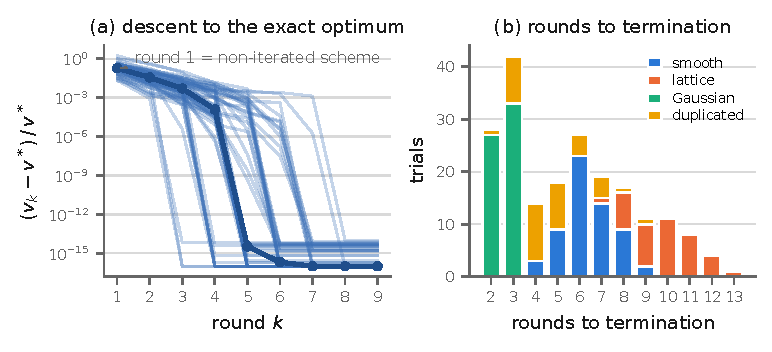
\includegraphics[width=\textwidth]{figs/convergence.pdf}
\caption{(a) Relative excess value $(v_k-v^*)/v^*$ per round for the 60
smooth-kernel trials (light curves; dark curve with markers: per-round
median), clipped at $10^{-16}$ for display. (b) Rounds to termination
across all 160 trials.}
\label{fig:convergence}
\end{figure}

Three observations connect the experiments to the theory. First, the
terminal agreement with the full-grid solve is at roundoff level in all
160 trials, including the duplicated-column suite, where supports may
legitimately differ while values and fits coincide
(Theorem~\ref{thm:outputs}). Second, from
Fig.~\ref{fig:convergence}a it is evident that the value sequence does
not decay asymptotically but drops by many orders of magnitude and then
\emph{terminates} at the roundoff floor --- the finite exact
termination of Theorem~\ref{thm:main}, as opposed to the geometric
convergence a contraction argument would suggest. Third, the
non-iterated scheme was suboptimal in every smooth-kernel trial, its
value exceeding the optimum by a median of 18\% (maximum 169\%);
therefore the feedback rounds carry the exactness in precisely the
correlated regime the method was designed for. Observed round
counts (2--9, median 3--6, Fig.~\ref{fig:convergence}b) are comparable
to the 3--7 refinement iterations reported in~\cite{brookes2006}. The
four-column instance of Proposition~\ref{prop:counter} is reproduced
exactly: single-pass value $\tfrac1{12}$, pricing violation
$\tfrac16$, and value $0$ after one refinement round.

\section{Discussion}\label{sec:discussion}

\paragraph{Lyapunov descent rather than contraction.}
A natural first approach is to show the round map contracts toward the
full solution. Two structural facts obstruct this: the fixed points of
the round map are exactly the global minimizers, which form a continuum
whenever the minimizer is non-unique, while a strict contraction on a
complete metric space has a unique fixed point; and no
instance-independent contraction factor exists, since ill-conditioned
(nearly parallel) columns make a single round's progress arbitrarily
small relative to the distance from the optimum. What survives, and
suffices, is that $F-v^*$ is a Lyapunov function for the round map ---
nonincreasing by Lemma~\ref{lem:mono}, strictly decreasing off the
solution set by Lemma~\ref{lem:strict}. Lyapunov descent alone would
give only asymptotic statements; the closing ingredient, particular to
this algorithm, is that every iterate is an exact minimizer over one of
finitely many column subsets, so the values live in a finite set and
strict descent must terminate. In this respect the method behaves like
the finitely terminating active-set algorithms it is built
from~\cite{lawson1974}, rather than like a fixed-point iteration.

\paragraph{Implementation guidance.}
The analysis identifies one implementation pattern as load-bearing.
Condition (H3) requires merges to union whole returned sets; a
multistage combining phase that re-partitions the unioned results into
fixed-size chunks --- a natural memory-management choice, and one
compatible with the description in \cite[\S4.1]{brookes2006} --- can
split a returned support across chunks, in which case
Lemma~\ref{lem:tree} no longer applies and a round can in principle lose
ground, taking the certificate's soundness proof with it. Since
returned sets are automatically small ($|U|\le\operatorname{rank}(A)$),
packing whole sets into stage groups costs nothing and preserves the
guarantee; this appears advisable in any implementation. Two further
practical consequences of the analysis: stopping on an unchanged
\emph{value} is sound and robust under non-uniqueness
(Remark~\ref{rem:stopping}), and logging the maximum pricing residual
per round turns Proposition~\ref{prop:inexact} into a per-run numerical
optimality certificate at negligible cost.

\paragraph{Limitations.}
The guarantee is stated for exact subproblem solves; floating-point
practice is covered only through the tolerance bound of
Proposition~\ref{prop:inexact}. The bound $K\le|V|$ on the number of
rounds is combinatorial, in the spirit of finite-termination results
for active-set and simplex methods, and we make no polynomial claim;
the observed counts are single digits, but a worst-case analysis
remains open. The analysis fixes the column set $S$: per-round
partitions may change, but enlarging or moving the grid itself between
rounds is a different algorithm and outside the present scope. Finally,
when systematic-noise elimination is interleaved between rounds as a
separate processing step, the objective changes from round to round and
the Lyapunov argument does not apply; this is consistent with the
report in~\cite{brookes2006} that the iterative variant need not reach
a fixed parameter set in that mode. If instead the noise degrees of
freedom are carried as sign-unconstrained columns in every subproblem
and solved jointly --- their optimality condition is plain
stationarity, and the pricing of the constrained columns is unchanged
--- the guarantee is restored.

\paragraph{Extensions.}
The proofs use only convexity and differentiability of $F$ together
with exact subproblem solves, so the theorem holds verbatim for
weighted least squares and other smooth convex losses. For
Tikhonov-regularized NNLS the augmented objective is strictly convex
when the regularizer has trivial kernel; minimizers are then unique and
the equivalence holds unconditionally at the level of the amplitude
vector itself, which is relevant to regularized variants of the
motivating analysis~\cite{brookes2010}. Overall, the results place the
production use of the iterated divide-and-conquer method on firm
footing and should support its transfer to other spectrum-type NNLS
applications where the parameter space exceeds single-node memory.

\section*{Declarations}

\paragraph{Funding.}
This work was supported by National Institutes of Health grant
R01~GM120600 (to E.H.B.).

\paragraph{Use of AI tools.}
During the preparation of this work the author used Claude (Anthropic)
in the development of the proofs, the verification software, and the
manuscript text. The author has reviewed and verified all mathematical
arguments and computational results and takes sole responsibility for
the content of this publication.

\paragraph{Data availability.}
The verification and experiment scripts (Python, using
\texttt{scipy.optimize.nnls}), together with the \LaTeX\ source of this
note, are available at \url{https://github.com/ehb54/nnls-dc-proof}.

\paragraph{Conflict of interest.}
The author declares no competing interests.

\bibliographystyle{abbrvnat}
\bibliography{refs}

\end{document}
